% =========================================================
% MÓDULO DE PERSISTENCIA (BASE DE DATOS)
% =========================================================
\section{Modelo de Persistencia}


En este capítulo se detalla la arquitectura de datos del sistema, incluyendo el diseño lógico y físico de la base de datos, así como las estrategias implementadas para garantizar la integridad y seguridad de la información. El diseño sigue el paradigma de mapeo objeto-relacional (ORM) a través de JPA/Hibernate, lo que permite una integración fluida entre la lógica de negocio en Java y el motor relacional PostgreSQL.

\section{Diagrama Entidad-Relación (DER)}
El diseño del modelo de datos sigue un enfoque relacional. A continuación se presenta la representación gráfica del modelo físico, el cual detalla las entidades, sus atributos y las relaciones de cardinalidad que rigen el flujo de información del sistema de denuncias.

\begin{figure}[htbp]
    \centering
    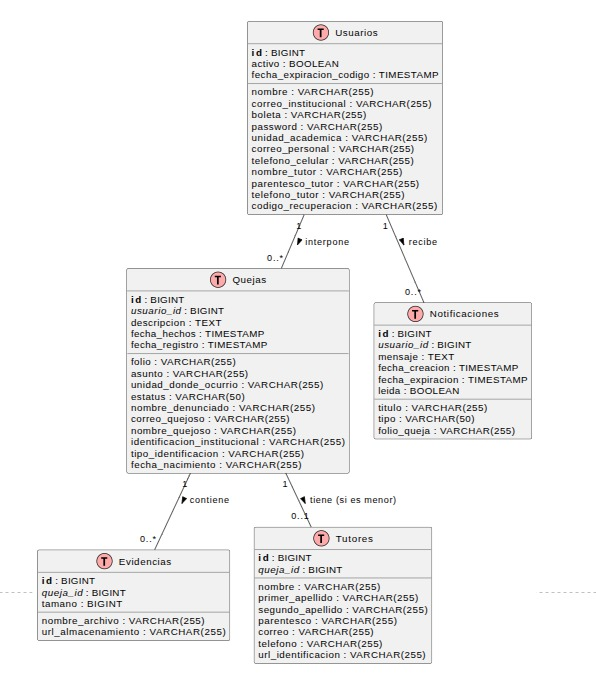
\includegraphics[width=0.9\textwidth]{imagenes/quejoso/basededatosquejoso.png} 
    \caption{Diagrama de Entidad-Relación del Sistema de Denuncia.}
    \label{fig:der_sistema}
\end{figure}

\section{Estrategia de Persistencia}
La persistencia de datos se gestiona mediante las siguientes definiciones tecnológicas:
\begin{itemize}
    \item \textbf{Motor de Base de Datos:} Se utiliza \textbf{PostgreSQL} para asegurar el cumplimiento de las propiedades ACID y la integridad referencial mediante claves foráneas.
    \item \textbf{Mapeo Objeto-Relacional (ORM):} Se emplea \textbf{Hibernate} a través de \textbf{Spring Data JPA}. Esto permite manipular los datos como objetos Java, reduciendo la probabilidad de errores en consultas SQL manuales.
    \item \textbf{Patrón Repository:} Se implementó este patrón para abstraer la capa de datos, facilitando la mantenibilidad y el intercambio de motores de base de datos en el futuro.
    \item \textbf{Seguridad:} Los datos sensibles, específicamente las contraseñas, se protegen mediante el algoritmo de hash robusto \textbf{BCrypt}.
\end{itemize}

% =========================================================
% MÓDULO BASE Y USUARIOS
% =========================================================
\section{Módulo de Usuarios y Autenticación}
La tabla \texttt{usuarios} constituye la entidad central para la autenticación y gestión de perfiles.

\subsection{Diccionario de Datos: Tabla Usuarios}
\begin{table}[H]
\centering
\small
\begin{tabularx}{\textwidth}{|l|l|l|X|}
\hline
\rowcolor{azulESCOM} 
\color{white}\textbf{Campo} & \color{white}\textbf{Tipo de Dato} & \color{white}\textbf{Restricciones} & \color{white}\textbf{Descripción} \\ \hline
id & BIGINT & PK, IDENTITY & Identificador único interno del registro. \\ \hline
correo & VARCHAR(255) & UNIQUE, NOT NULL & Correo institucional del usuario. \\ \hline
password & VARCHAR(255) & NOT NULL & Hash criptográfico de la contraseña (BCrypt). \\ \hline
boleta & VARCHAR(50) & UNIQUE, NOT NULL & Identificador institucional (alumno o empleado). \\ \hline
nombre & VARCHAR(255) & - & Nombre(s) del titular del perfil. \\ \hline
reset\_token & VARCHAR(255) & UNIQUE & Token para la recuperación de la cuenta. \\ \hline
\end{tabularx}
\caption{Diccionario de datos de la entidad \texttt{usuarios}.}
\label{tab:dict_usuarios}
\end{table}

\subsection{Implementación de la Entidad (JPA)}
\begin{lstlisting}[language=Java, caption={Entidad Java para la gestión de usuarios.}, label={lst:java_usuario}]
@Entity
@Table(name = "usuarios")
@Data
public class UsuarioEntity {
    @Id
    @GeneratedValue(strategy = GenerationType.IDENTITY)
    private Long id;

    @Column(unique = true, nullable = false)
    private String correo;
    
    @Column(nullable = false)
    private String password;
    
    @Column(unique = true, nullable = false, length = 50)
    private String boleta;
    
    private String nombre;
    private String primerApellido;
    private String segundoApellido;
}
\end{lstlisting}

% =========================================================
% MÓDULO DE FOLIOS Y EVIDENCIAS
% =========================================================
\section{Módulo de Gestión de Folios y Evidencias}
La entidad \texttt{FolioEntity} constituye el núcleo de información de la plataforma, consolidando los datos del incidente y los archivos probatorios.

\subsection{Diccionario de Datos: Tabla Folios}
\begin{table}[H]
\centering
\small
\begin{tabularx}{\textwidth}{|l|l|l|X|}
\hline
\rowcolor{azulESCOM} 
\color{white}\textbf{Campo} & \color{white}\textbf{Tipo de Dato} & \color{white}\textbf{Restricciones} & \color{white}\textbf{Descripción} \\ \hline
id & BIGINT & PK, IDENTITY & Identificador interno. \\ \hline
codigo\_folio & VARCHAR(255) & UNIQUE, NOT NULL & Folio público de seguimiento. \\ \hline
asunto & VARCHAR(255) & NOT NULL & Título descriptivo de la queja. \\ \hline
descripcion & TEXT & - & Detalle de los hechos denunciados. \\ \hline
nombre\_tutor & VARCHAR(255) & - & Nombre del tutor (en caso de menores). \\ \hline
\end{tabularx}
\caption{Diccionario de datos de la entidad Folios.}
\label{tab:dict_folios}
\end{table}

\subsection{Gestión de Evidencias Digitales}
La tabla \texttt{evidencias} registra la ubicación de los archivos en el servidor, vinculándolos directamente a un folio mediante una relación de "Uno a Muchos".

\begin{lstlisting}[language=SQL, caption={Script DDL para la tabla de evidencias.}]
CREATE TABLE evidencias (
    id BIGSERIAL PRIMARY KEY,
    nombre_archivo VARCHAR(255) NOT NULL,
    ruta_almacenamiento VARCHAR(500) NOT NULL,
    folio_id BIGINT NOT NULL,
    CONSTRAINT fk_folio_evidencia FOREIGN KEY (folio_id) 
        REFERENCES folios(id) ON DELETE CASCADE
);
\end{lstlisting}

% =========================================================
% MÓDULO DE SEGUIMIENTO (QUEJAS E HITOS)
% =========================================================
\section{Módulo de Seguimiento de Quejas}
Este módulo permite la trazabilidad cronológica de cada expediente mediante el uso de estados e hitos.

\subsection{Diccionario de Datos: Tabla Quejas y Hitos}
Para garantizar que cada avance sea registrado, se utiliza la tabla \texttt{queja\_hitos}, la cual almacena cada cambio administrativo realizado sobre una queja.

\begin{table}[H]
\centering
\small
\begin{tabularx}{\textwidth}{|l|l|l|X|}
\hline
\rowcolor{azulESCOM} 
\color{white}\textbf{Campo} & \color{white}\textbf{Tipo de Dato} & \color{white}\textbf{Restricciones} & \color{white}\textbf{Descripción} \\ \hline
folio & VARCHAR(255) & PK & Identificador alfanumérico único. \\ \hline
status & VARCHAR(50) & DEFAULT 'PENDIENTE' & Estado actual del proceso. \\ \hline
fecha\_inicio & TIMESTAMP & DEFAULT NOW() & Fecha de registro inicial. \\ \hline
\end{tabularx}
\caption{Diccionario de datos de la entidad Quejas.}
\end{table}

% =========================================================
% CATÁLOGOS Y ORDEN
% =========================================================
\section{Catálogos del Sistema y Scripts de Creación}
Para estandarizar la clasificación, se implementan catálogos de \textbf{Estatus}, \textbf{Temas} y \textbf{Tipos de Documento}. El orden de ejecución de los scripts DDL es crítico para mantener la integridad referencial:

\begin{enumerate}
    \item \texttt{cat\_estatus\_queja}, \texttt{cat\_tema}, \texttt{cat\_tipo\_documento} (Catálogos base).
    \item \texttt{usuarios} y \texttt{folios} (Entidades principales).
    \item \texttt{quejas}, \texttt{evidencias} e \texttt{hitos} (Dependencias funcionales).
    \item \texttt{notificaciones} y tablas auxiliares.
\end{enumerate}

\begin{center}
\fbox{\parbox{0.9\textwidth}{\centering\textbf{Nota sobre Rendimiento:} Se han creado índices sobre las columnas \texttt{folio}, \texttt{boleta} y \texttt{usuario\_id} para optimizar la velocidad de búsqueda en procesos con grandes volúmenes de datos.}}
\end{center}